The DARPA-funded project \emph{High Assurance Cyber-Military System (HACMS)} aims to produce systems and software with proved reliability and security.
Systems designed at SRI as part of this project are inspired by the ROS (Robot Operating System) architecture.
In ROS, we use the abstraction of \textit{nodes} and \textit{topics} to describe the different components and communication channels. 
At initialization, each node is declared subscriber to some topics and publisher on others. At each step, a node reads messages from the subscribed topics, execute a computation and publish on the topics it is in charge.

Each node is set to execute at a given frequency, but the actual rate to publish messages may vary because of clock bias, or a computing duration depending on the inputs. Since several nodes may execute physically on the same processor, scheduling randomness adds to this imprecision. 
When a message is published on a topic, it may need a certain delay before it is received by the subscribers. This delay is caused by the nature of the communication link (network/shared memory) and the underlying mailbox system.
For these reasons, we cannot ensure a subscriber will have new messages at each step, or that sent messages will be processed by the subscriber (they may be overridden before that).
Figure~\ref{msg} gives examples for these problems.

\begin{figure}[h]
\begin{center}
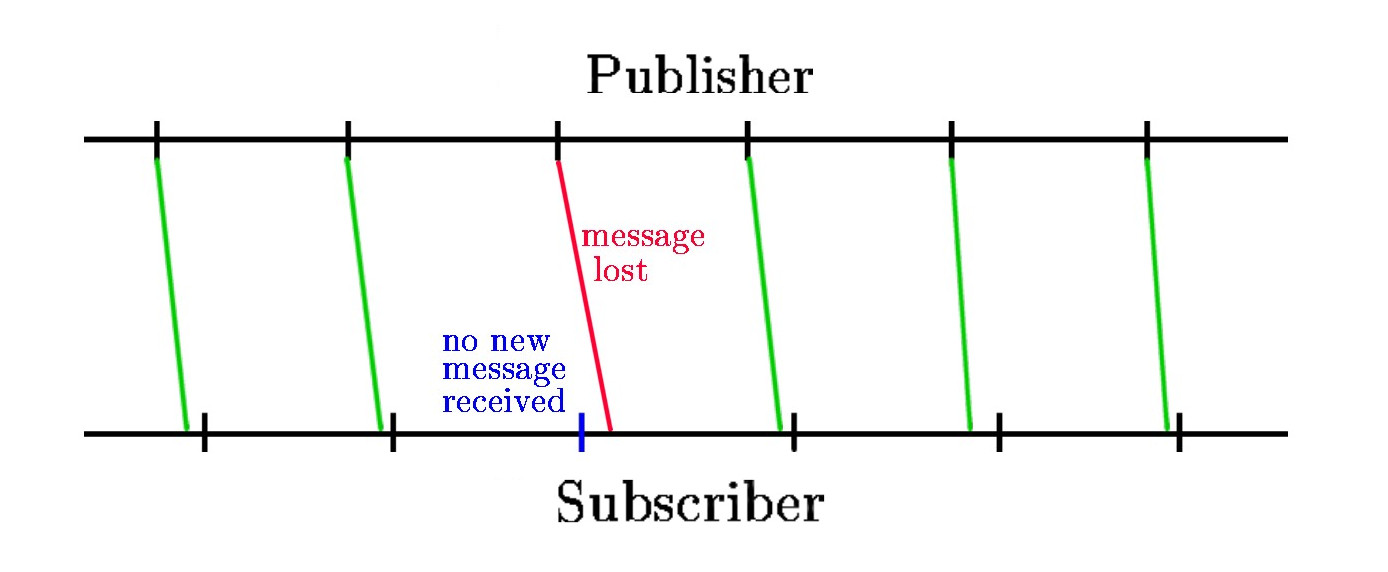
\includegraphics[height=6cm]{messages.jpg}
\caption{Uncertainty for the messaging system}\label{msg}
\end{center}
\end{figure}


In this report, we will establish a worst case scenario for this messaging system. For example, knowing that a node will always have available at least one message with a bounded age can be sufficient to assert a control loop maintains a state precisely enough around the desired value.
This can also be used for monitoring purposes: if a node detects a behavior outside this worst case scenario, it can raise an alert to a supervisor. By collecting these alerts, the supervisor could detect a compromised/crashed node, or a broken link, and decide how to fix the problem.

In Section 3, we give more details about the ROS architecture and the model used to represent it. In Section 4, we prove low-level properties for the messaging system. In sections 5 to 7, we give assurance claims for simple end-to-end properties. Section 5 proves that a basic control loop maintains a state around a set value. Sections 6 and 7 give two different models for obstacle avoidance.